
\setchapterpreamble[u]{\margintoc}
\chapter{Communicating with your microcontroller}
\labch{connect}

The purpose of this book is to provide you with the necessary skills and experience to design, build and use instruments to measure environmental conditions.
The ``brain'' of these instruments is a \emph{microcontroller}.
A microcontroller is a device with a processing unit that can run codes and other instructions, and external connections (called \emph{pins}) to transmit electrical inputs and outputs.
The microcontroller is what enables your instrument to receive information from sensors, monitor and regulate its power supply, and communicate for receiving instructions and telemetering data.
Learning to communicate with and control a microcontroller is the first step in building and using environmental sensing instruments.

There are many types of microprocessors, which vary by overall size, power requirements, capabilities to input and output different kinds of electrical signals, onboard communication hardware like WiFi or USB, and the types of code or instructions they accept.
%
This textbook focuses on microprocessors that use instructions written in \htmladdnormallink{MicroPython}{https://micropython.org/}, a subset of the \htmladdnormallink{Python}{https://www.python.org} programming language.
MicroPython is a recent invention, and a great improvement for learning about, building and using environmental sensors.
Because MicroPython-based microcontrollers are automatically interactive
\sidenote[][3cm]{\begin{kaobox}[backgroundcolor=\SNcolor,frametitlebackgroundcolor=\SNcolor,frametitle=MicroPython is \texttt{REPL}-ent!]Like Python, MicroPython runs in an interactive session.
	This session goes by the  technical-sounding name \textbf{REPL}, which stands for ``Read-Evaluate-Print-Loop''.
%	, or \emph{REPL}.
	Despite this name, REPL is a very intuitive interface.
	REPL simply means that, in a MicroPython (or Python) session, you type commands, which are then executed, and the results are displayed.
\end{kaobox}}
, they are good platforms for learning to develop and debug codes to collect data from environmental sensors.

Python itself is a powerful and easy to learn language for scientific computing on desktops and laptops.
If you already know some Python, you can apply that knowledge to working with MicroPython-based microcontrollers.
If you're new to Python, then by learning MicroPython you will simultaneously learn how to use Python for many other tasks.
%In fact, m
Many of the exercises in this book combine acquiring data from sensors using a microcontroller, and analyzing or plotting those data on a computer, using the same Python coding language.

%\marginnote[3cm]{Note that Python is currently undergoing a transition, from an older version (Python 2.7) to newer Python 3 versions.
%These are mostly similar, but differ in some details such as the syntax of print commands. Because MicroPython is based on Python 3, and because older versions of Python will soon no longer be supported, the codes and instructions in this book will use Python 3.}
%In most cases, Python 2.7 users will need to make only minor adjustments.
\begin{kaobox}[frametitle=Once and future Python]
	Note that Python is currently undergoing a transition, from an older version (Python 2.7) to newer Python 3 versions.
	These are mostly similar, but differ in some details such as the syntax of print commands. Because MicroPython is based on Python 3, and because older versions of Python will soon no longer be supported, the codes and instructions in this book will use Python 3.
\end{kaobox}


\begin{table}[h]%[2cm]
	\caption[\refch{connect} materials]{\textbf{Materials you'll need\dots}
%	\caption[	\textbf{\refch{connect} blah Materials you'll need\dots}
		See Table \ref{tab:materials} for additional information.}%]

		\labtab{materials_connections}
\begin{center}
			\raggedright
		%\begin{tabular}{ c c c c }
		\begin{tabular}{ c r c}
			\hline
			Sections & item & link \\
			\hline
			\multirow{3}{4em}{\refsec{connections}}
			& breadboard & \ref{mat:bb} \\
			& ESP8266 ``Feather'' & \ref{mat:mc} \\
			& micro-USB cable & \ref{mat:usb_cbl} \\
			\hline
			\multirow{1}{4em}{\refsec{WiFi_connect}}
			& WiFi router & \ref{mat:router} \\
			& WiFi USB dongle & \ref{mat:dongle} \\
			\hline
		\end{tabular}

\end{center}

\end{table}



%\section{Meet your microcontroller}
%\labsec{microcontrollers}

\subsubsection{Meet your microcontroller}
%\subsubsection{How to use this book}


For examples in this book, we will use Adafruit's Feather HUZZAH ESP8266 microcontroller.
It is small, has built-in WiFi, uses relatively little power, and is low cost for its capabilities.
The core ESP8266 microcontroller was originally intended to be placed in ``smart'' lightbulbs.
\sidenote[][*-7]{\begin{kaobox}[backgroundcolor=\SNcolor,frametitlebackgroundcolor=\SNcolor,frametitle=Lighten up!]See \htmladdnormallink{Tinnkerman's light bulb hacks}{https://tinkerman.cat/post/yet-another-wifi-light-bulb/} for some fun examples in which the ESP8266 microcontroller is reprogrammed in place within a smart light bulb.
Very large scale production for this purpose has made this microcontroller inexpensive, which also makes it a good choice for putting in sensors in often-harsh environments.\end{kaobox}}
Many of the characteristics designed for its intended purpose also make it suitable for environmental sensing instruments.

Note that the exercises in this book can be successfully completed using other microcontrollers.
We focus here on the Feather ESP8266 because it's one of the microcontrollers officially supported by \htmladdnormallink{MicroPython}{https://http://micropython.org/}, because Adafruit provides good documentation and support for it, and because it's likely to be available for some time into the future.
The other officially supported microcontroller, Adafruit's HUZZAH ESP8266 Breakout Board, is slightly smaller and cheaper, but requires a special cable for communications rather than a generic microUSB cable.
Other manufacturers also make microcontroller boards based on the ESP8266.
Many of these will work in essentially the same way for exercises in this book.
Boards using other processors also can work.
These alternative microcontrollers may require modifying details in the MicroPython codes, such which connections are used for electrical inputs and outputs.
The \htmladdnormallink{MicroPython}{https://http://micropython.org/} website is the best reference if you are considering using alternative microprocessor boards for the activities in this book.

\begin{marginfigure}[2cm]
	\begin{center}
		\htmladdnormallink{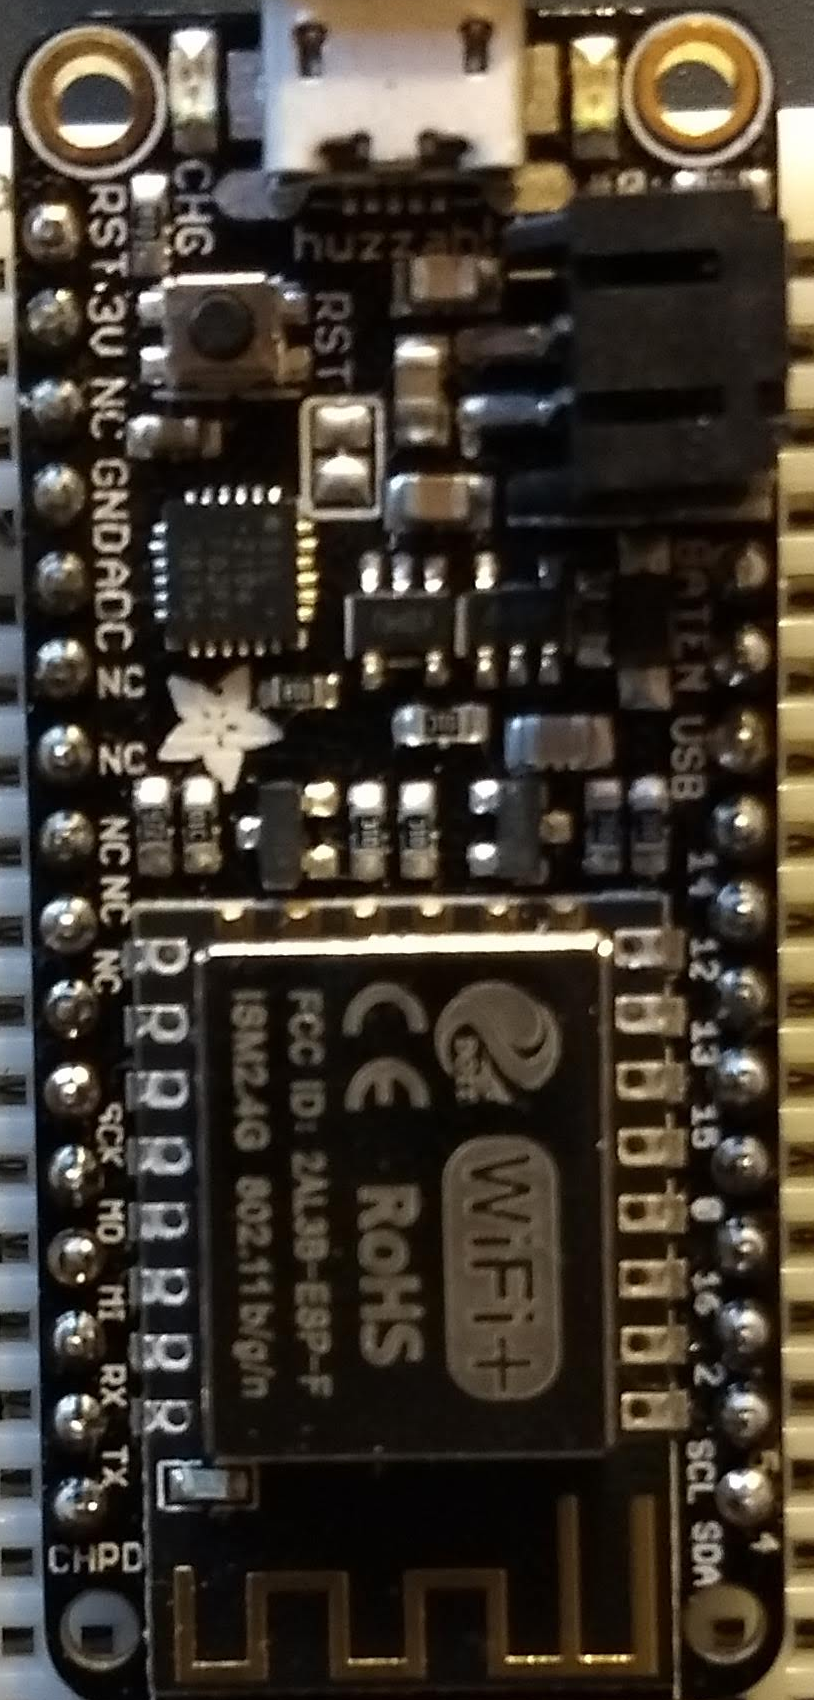
\includegraphics[width=\MFW]{Images/ESP8266feather_top.png}}{https://publicsensors.org/IntroSensors/Images/ESP8266feather_top.png}
		\caption[ESP8266 feather microcontroller]{A ESP8266 Feather microcontroller.}
		\labfig{margin_esp8266}
	\end{center}
\end{marginfigure}

A close-up view of the ESP8266 Feather (\reffig{margin_esp8266}) shows the key features we will use to create functional environmental sensors.
\marginnote[-3.5cm]{
	The documents \htmladdnormallink{adafruit-feather-huzzah-esp8266.pdf}{https://cdn-learn.adafruit.com/downloads/pdf/adafruit-feather-huzzah-esp8266.pdf} and \htmladdnormallink{adafruit-huzzah-esp8266-breakout.pdf}{https://cdn-learn.adafruit.com/downloads/pdf/adafruit-huzzah-esp8266-breakout.pdf} are the best overall resources for information about the Adafruit Huzzah Feather and Breakout versions of the ESP8266 microcontroller.
	Please download the document for your microcontroller for future reference about specifications, pin definitions, voltage tolerances, \etc
}
The core microcontroller is the rectangular component near the bottom.
The zigzag line below it is a built-in WiFi antenna.
At the top is a connector for a microUSB cable, used to communicate with the Feather.
Plugging a USB cable into this connector and into your computer automatically supplies power to the microcontroller.
It also automatically supplies a connection for communicating with the microcontroller.% -- see \refsec{usb_connect} for instructions on how to use USB to communicate with your microcontroller.

Below and to the left of the USB connector is a button, labelled ``\texttt{RST}''.
This is a reset button, used occasionally to halt a run-away code or reboot a malfunctioning microcontroller (normally we will do this via software, so we rarely need to use the \texttt{RST} button).
At the four corners are holes for mounting screws.
Along the right and left edges are soldered ``pins'', %which are spaced to fit into a breadboard, and
which have different capabilities to transmit electrical signals to and from the microcontroller.
These pins have labels alongside (sometimes a little above or below) that identify the pin, so it can be referred to in MicroPython codes.
We will explain how to use these pins in \refch{first_exercises}.

\begin{kaobox}[frametitle=A flash of insight]
	In these exercises, we assume that your microcontroller already has the basic software needed to run MicroPython. This basic software is called ``firmware'', which must be ``flashed'' onto a microcontroller. The instructions for flashing MicroPython firmware onto your microcontroller are given at the \htmladdnormallink{Getting started with MicroPython}{http://docs.micropython.org/en/latest/esp8266/tutorial/intro.html\#intro} tutorial. If your microcontroller doesn't yet have its firmware, follow the instructions in that tutorial to get ready for the activities in this book.
\end{kaobox}



%\begin{marginfigure}[0cm]
%	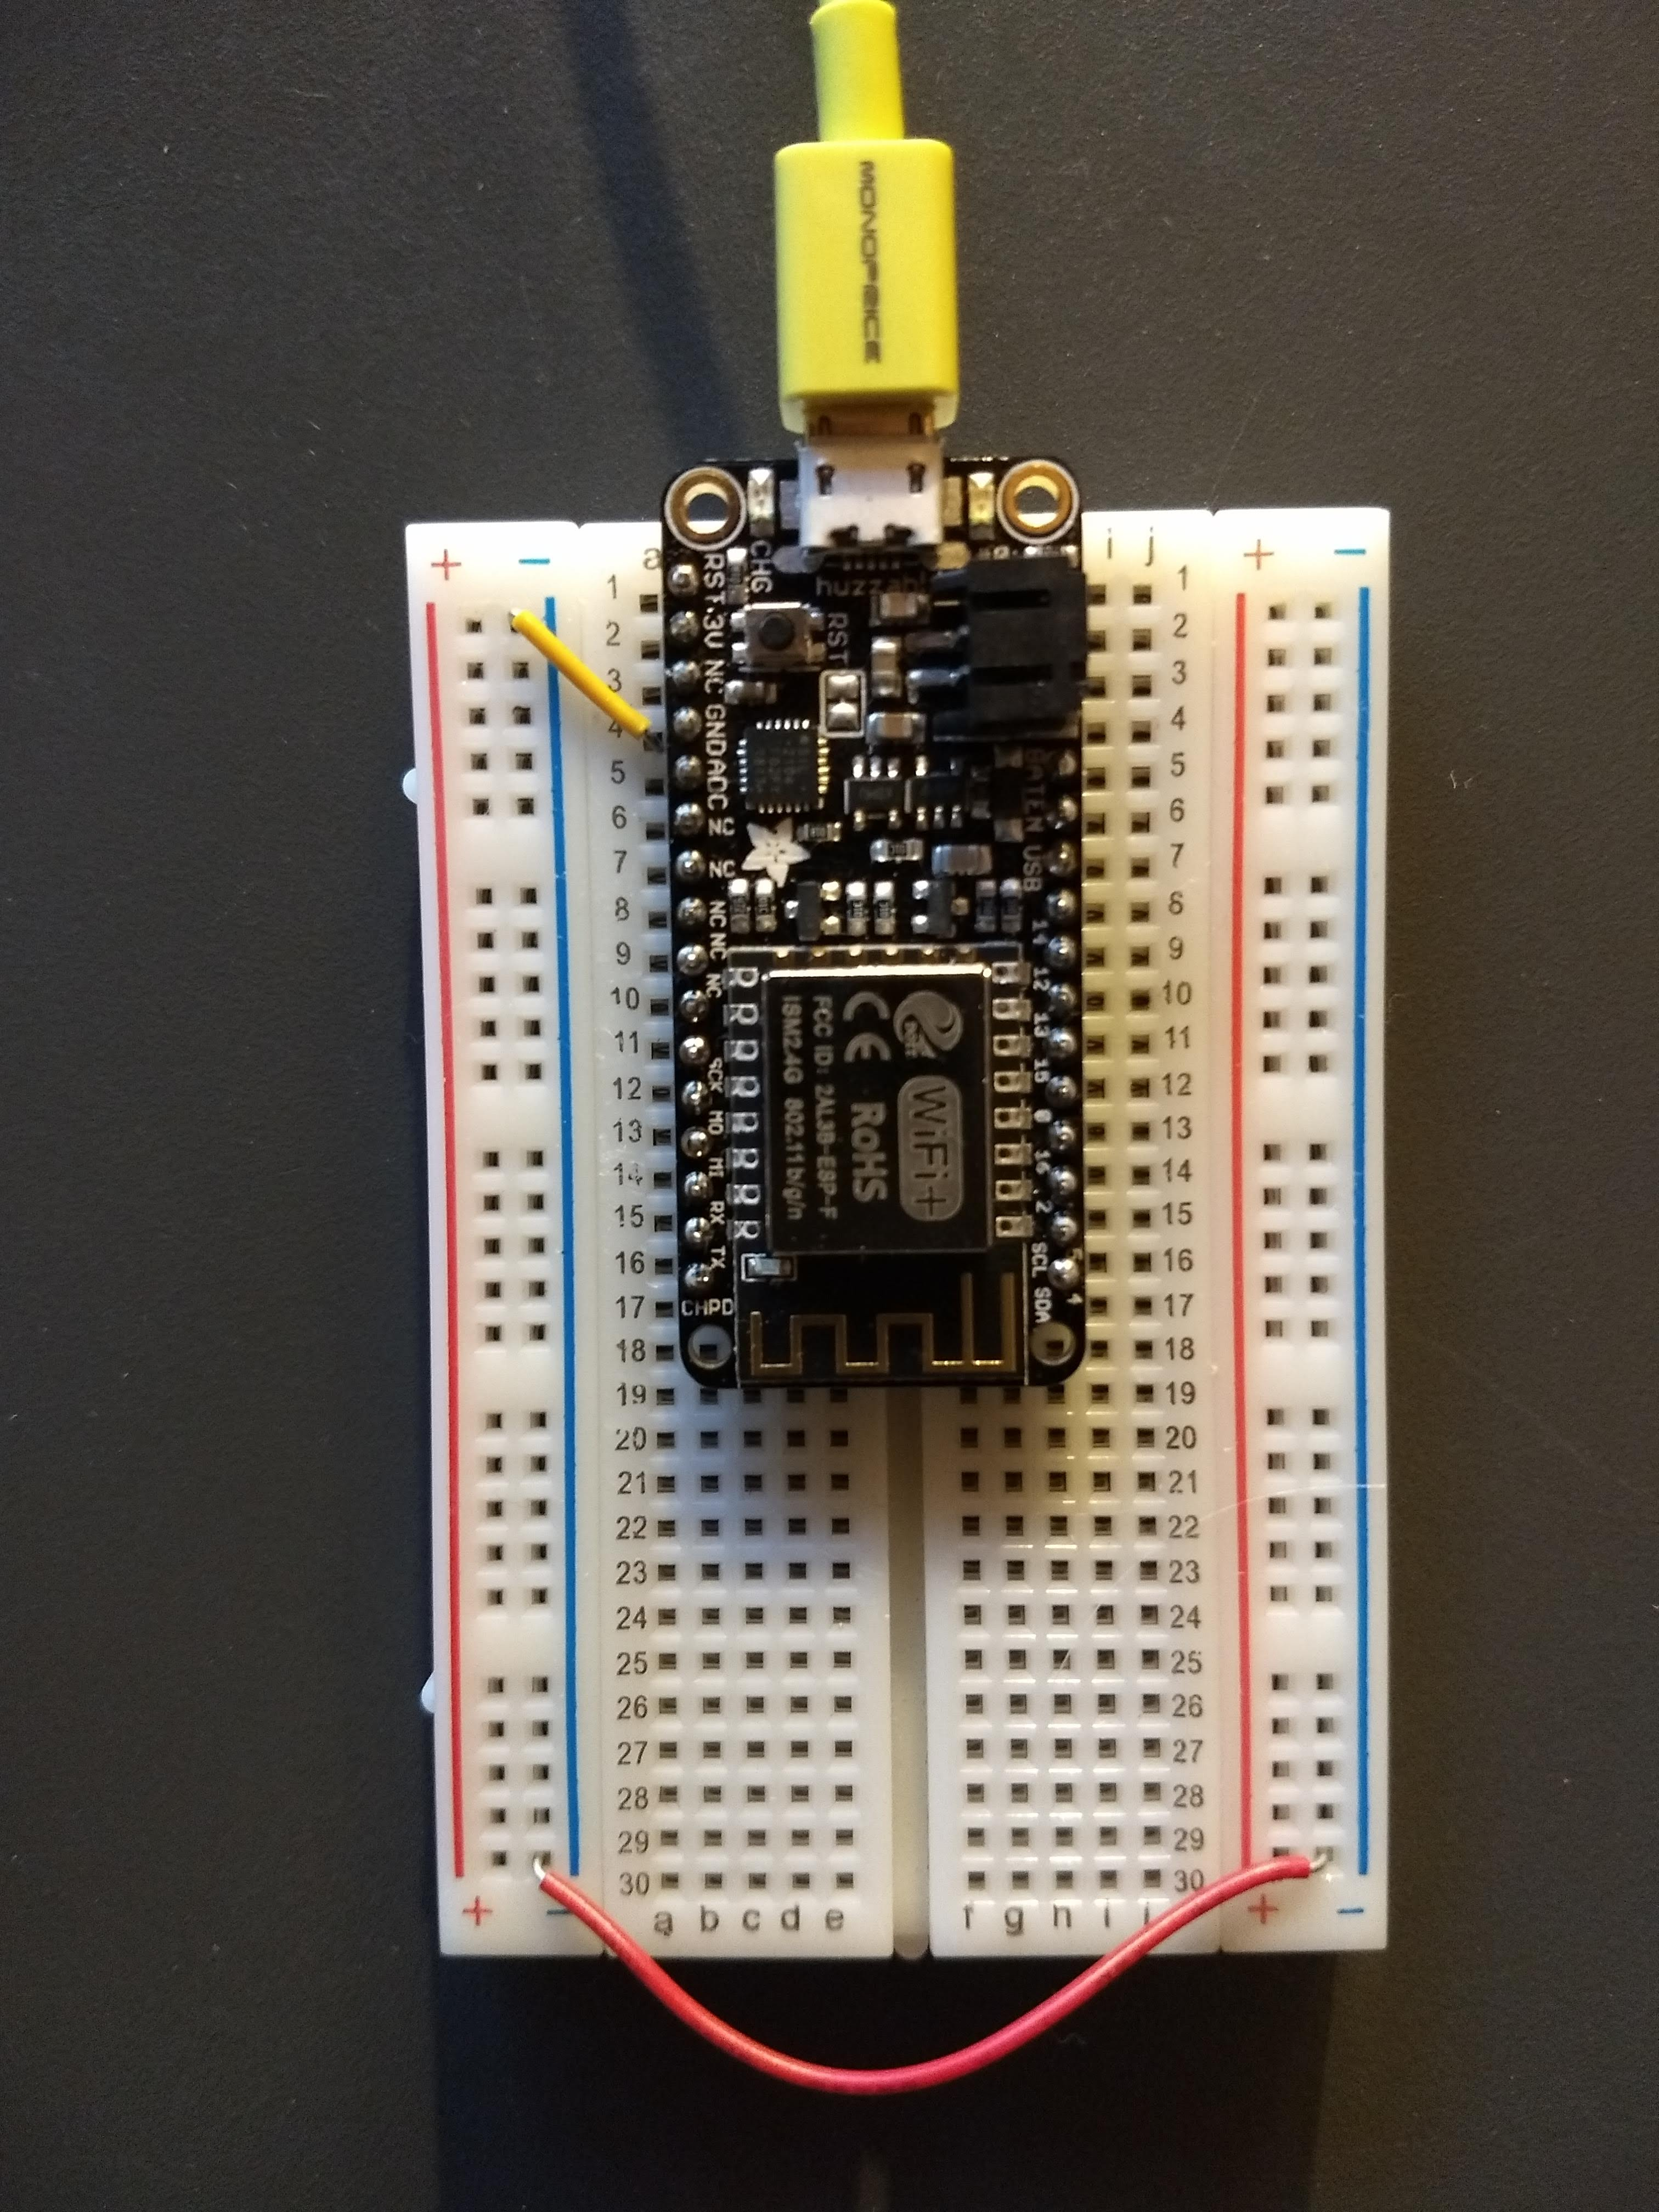
\includegraphics{Images/breadboard_ESP8266feather.jpg}
%	\caption[ESP8266 feather microcontroller on breadboard]{Breadboard with ESP8266 feather.}
%	\labfig{margin_breadboard_esp8266}
%\end{marginfigure}

%%
%%\begin{lstlisting}
%%	\begin{marginfigure}
%%		\includegraphics{Images/IMG_20181205_082817686.jpg}
%%		\caption[ESP8266 feather microcontroller on breadboard, too]{Breadboard with ESP8266 feather, again.}
%%		\labfig{esp8266brd}
%%	\end{marginfigure}
%%\end{lstlisting}
%

\section{Establishing communications}
\labsec{connections}

Our starting point for building and using environmental instruments is learning how to communicate with microcontrollers from your desktop or laptop computer.
The ESP8266 Feather (and many other microcontrollers) have two primary modes of communication: USB and WiFi.
Some microcontrollers have additional communication modes, such as BlueTooth, LoRa or other wireless protocols.
However, USB and WiFi are the most common, standardized and useful communication modes for microcontrollers, so in this book we focus on these two modes.

In general, either USB or WiFi mode alone can be sufficient for building and using environmental sensors.
However, it is often very helpful to have both options.
For example, WiFi connections can be very useful when working with microcontrollers in environmental sensing instruments, which are often deployed inside waterproof housings that make it impossible to connect a cable.
On the other hand, when generating and debugging codes to run these instruments, it is frequently necessary to reboot the microcontroller.
This breaks the WiFi connection, so that the REPL session (and usually the WiFi connection itself) must be re-initiated.
In this case a USB connection, which remains active through the reboot, may be more convenient.

To work efficiently and effectively with microcontrollers, we require two essential communication functions:
\begin{enumerate}
	\item We need to issue commands and see output during a REPL session; and,
	\item We need to transfer files, such as MicroPython codes and environmental data, on and off the microcontroller's flash memory.
\end{enumerate}
Both these functions can be accomplished using either USB or WiFi.

Below, we describe two alternative approaches for communicating with  ESP8266 microcontrollers running MicroPython. Both are free, and can be implemented on most desktop and laptop computers.
\begin{itemize}
	\item Google's Chrome browser, with extensions enabling communications via USB and WiFi.
	\item \mpfshell, a command line utility (that is, a small Python script that works within a simple terminal window).
\end{itemize}
Of the two, the Chrome browser approach has the advantages that it is very easy to install on most computers, and it looks and acts very much the same across Windows, Mac OS, Chromebooks and linux computers.
However, the Chrome browser interface is slower and in some ways less capable.
Also, the only browser-based method currently available to transfer files to/from the microcontroller is through WiFi (using WebREPL, described below).

\mpfshell can both support a REPL session and transfer files, over either USB or WiFi.
The \mpfshell approach requires that Python be installed on your computer, if it is not already
(Mac OS and linux machines have Python pre-installed, but many Windows users must install it, and \mpfshell is not available for Chromebooks).
While this installation may require some extra effort, working with microcontrollers through \mpfshell is so much more effective that we recommend you take this approach whenever possible.


%\marginnote[0cm]{
\begin{kaobox}[frametitle=As you get started \dots]
One of the challenges in working with microcontrollers is that the first step -- establishing communications -- is often the fussiest part of the entire process.
That is because, while the microcontrollers are relatively standardized, the computers we use to communicate with them have highly variable and frequently changing hardware and software.
These variations may results in differences in drivers, ports and communications software between.
\emph{It's important to approach this first step patiently and systematically, and to be prepared to ask for help from experienced people in person or online.}
In addition to the instructions in this chapter, tutorials for setting up and troubleshooting USB and WiFi connections can be found at the \htmladdnormallink{MicroPython}{https://micropython.org/} website and many other resources online.
\end{kaobox}
%}


\section{Connecting to your microcontroller via USB}
We will first take you through the steps necessary to connect to your microcontroller using USB. In \refsec{WiFi_connect}, we will use this USB connection to set up your microcontroller for WiFi connections.

\subsection{Installing drivers for USB connections}
If your laptop runs Windows, OS X (Mac) or Chrome OS, you may need to install a driver to enable your computer to connect with serial USB converter on your ESP8266 Feather microcontroller (this is not needed on linux machines).
The driver is available at \htmladdnormallink{this link}{https://www.silabs.com/products/mcu/Pages/USBtoUARTBridgeVCPDrivers.aspx}.
%\todo{This link is now broken.}

Computers with older operating systems may require an older version of the driver.
If you install the newest one and still cannot connect to the microcontroller, try installing the next older one.
Note that you must \emph{uninstall} the existing driver version \emph{before} installing a different version.
Instructions are included in the downloaded package files, and on the download website.

\subsection{USB connections via the Chrome browser}
If you will use the Chrome browser for your microcontroller work, you can install it from Google's \htmladdnormallink{download page}{https://www.google.com/chrome/}.
For USB connections, you need to install an extension called \textbf{BeagleTerm}.
From a Chrome browser window, navigate to  \htmladdnormallink{this link}{https://chrome.google.com/webstore/detail/beagle-term/gkdofhllgfohlddimiiildbgoggdpoea?hl=en}, and use the button at the upper right to install it.
BeagleTerm will now appear in your list of \htmladdnormallink{Apps}{chrome://apps/}.

\begin{marginfigure}[-18cm]
	\begin{center}
		\htmladdnormallink{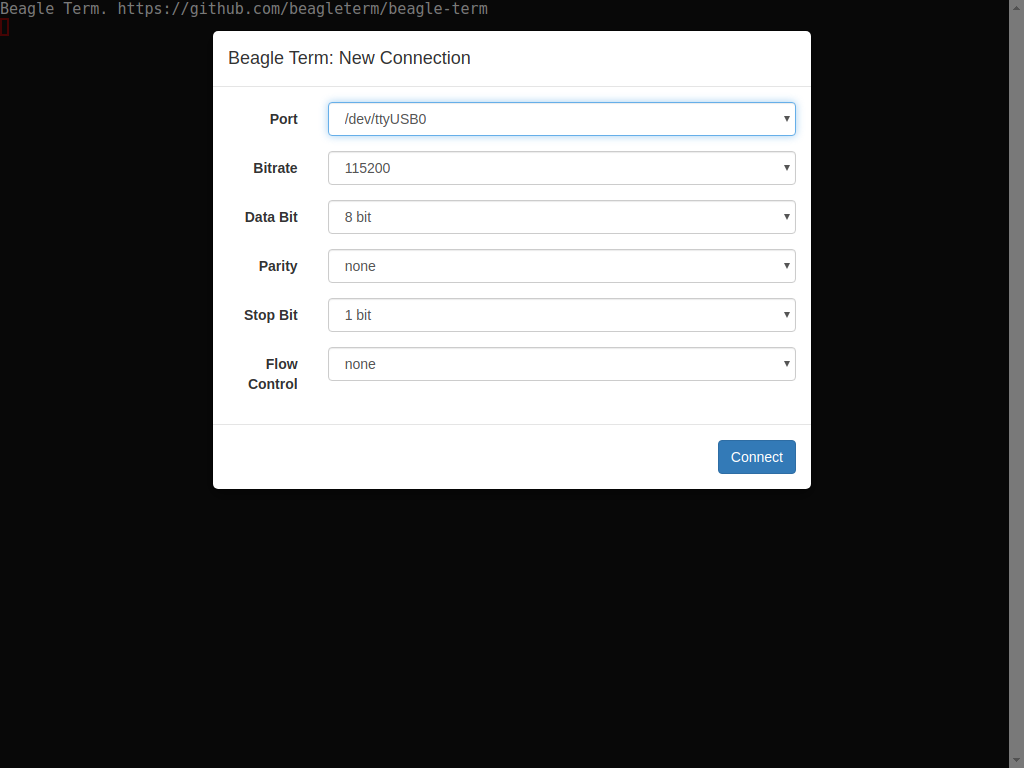
\includegraphics[width=\MFW]{Images/BeagleTermConnect.png}}{https://publicsensors.org/IntroSensors/Images/BeagleTermConnect.png}
		\htmladdnormallink{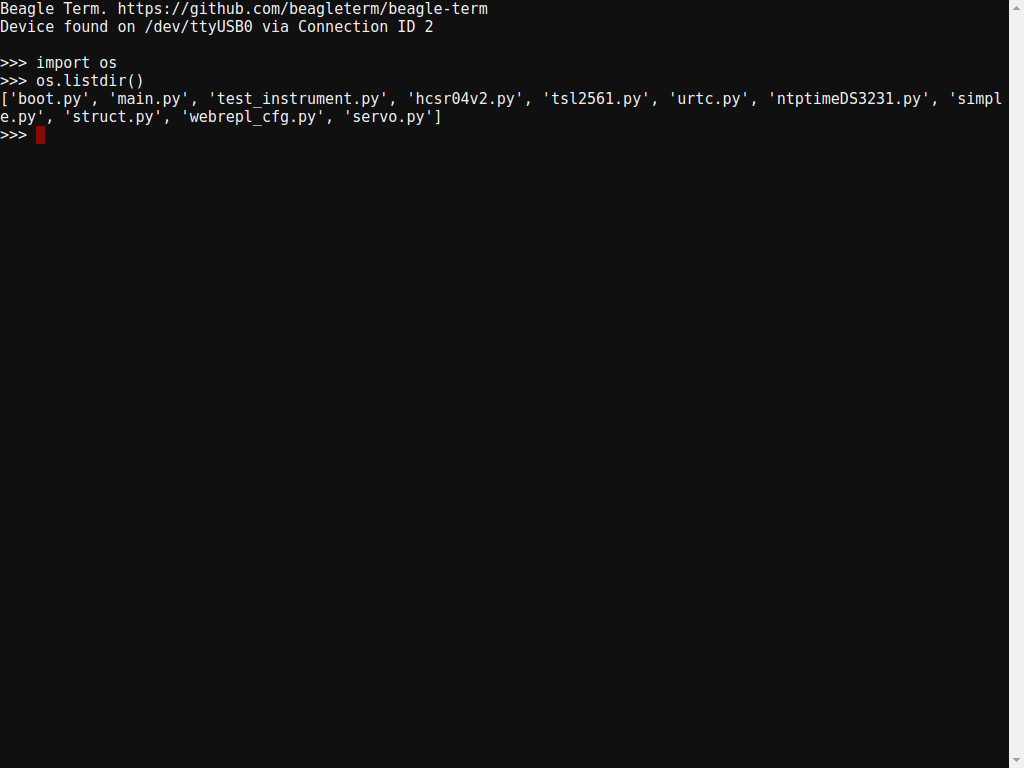
\includegraphics[width=\MFW]{Images/BeagleTerm.png}}{https://publicsensors.org/IntroSensors/Images/BeagleTerm.png}
%		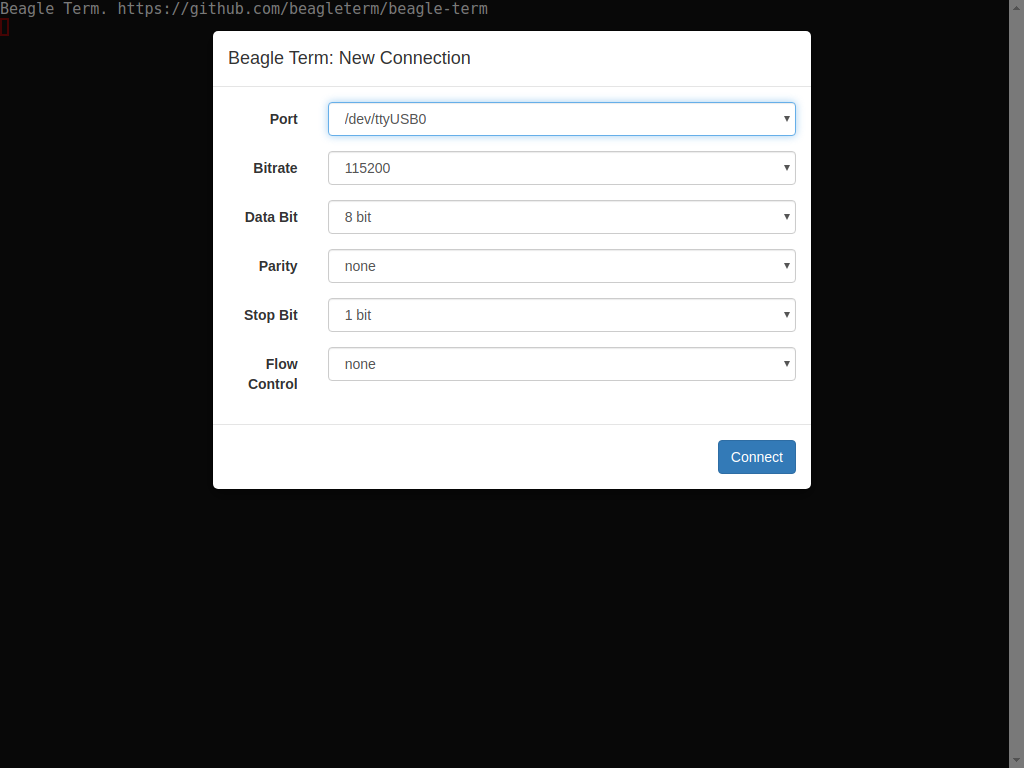
\includegraphics[width=5cm]{Images/BeagleTermConnect.png}
		\caption[Connection via BeagleTerm.]{BeagleTerm browser windows. Upper screenshot: The connection prompt with settings. Most of these default into the correct values. The Com port setting, in this case \texttt{ttyUSB0}, is the most likely one you may need to change. Lower screenshot: After connecting, press \texttt{return} on your keyboard to start a REPL session.}
		\labfig{BeagleTermConnect}
	\end{center}
\end{marginfigure}

\subsubsection{\howto{} Connect to your microcontroller via BeagleTerm}
\begin{enumerate}
	\item \textbf{Plug a USB cable into your computer and your microcontroller (before you launch BeagleTerm)}.
	\item \textbf{Launch the BeagleTerm app.}

	Usually the default parameters are correct, if the USB cable is already connected to both the computer and microcontroller when the app launches (\reffig{BeagleTermConnect}).
	\item \textbf{Click ``Connect'' and press ``Enter'' a couple times on your keyboard.}

	You should now see a ``\verb|>>>|'' Python prompt, meaning you are connected and ready to work with your microcontroller.
\end{enumerate}
If this does not work, the culprit is usually the ``Com port'' setting.
Use the menu to try the available ports until you find the right one.

%Note that there is currently no way (other than copying and pasting) to transfer files between your computer and microcontroller via a USB cable.
\subsection{\color{gray}USB connections via \thonny \color{black}}

\subsubsection{\color{gray}\howto{} Install and connect to your microcontroller via \thonny \color{black}}





\subsection{USB connections via \mpfshell}
\mpfshell is a Python-based file explorer and serial communications package.
We have found \mpfshell to be the most convenient utility for communication with ESP8266-based microcontrollers, because it includes both key communications functions.
Users can rapidly switch between interactive REPL sessions and file transfers, with a few keystrokes.
\mpfshell also works over both USB and WiFi.

%\subsubsection{To install \mpfshell:}
\subsubsection{\howto Install \mpfshell}

Instructions for installing and using \mpfshell are at \htmladdnormallink{this link}{https://github.com/wendlers/mpfshell}.
\mpfshell requires that Python be installed on your computer, preferably the most recent version (currently 3.5.9).
Machines running OS X or linux have Python pre-installed.
See links at \htmladdnormallink{Python}{https://www.python.org/downloads/windows/} and \htmladdnormallink{mpfshell}{https://gist.github.com/hardye/657385210c5d613e69cb5ba95e8c57a7} for instructions on installing Python and \mpfshell on Windows machines.
\begin{kaobox}[frametitle=Using \mpfshell in \htmladdnormallink{Integrated Development Environments}{https://en.wikipedia.org/wiki/Integrated_development_environment}  (\texttt{IDE}s)]
	\mpfshell generally works when installed and used within a \python \texttt{IDE} such as \htmladdnormallink{Enthought Canopy}{https://assets.enthought.com/downloads/}.
	\python \texttt{IDE}s can have advantages in generating and debugging code.
	However, in some cases, we have found that functions such as copying and pasting text in \texttt{REPL} sessions have been more limited within an \texttt{IDE} session than when running Python within a simple terminal.
	When possible, therefore, we recommend running \mpfshell from a simple terminal, even if you like to edit code from within an \texttt{IDE}.
\end{kaobox}

With Python3 installed, the \texttt{pip3} utility makes it straightforward to install \mpfshell and a few other Python packages it requires on Mac OS and linux computers:
\begin{enumerate}
	\item \textbf{Open a terminal window.}
	\item \textbf{Install the latest version of \mpfshell and the packages it requires.}

	On Mac OS and linux machines, use a terminal window to issue the command\sidenote[][*-8]{\begin{kaobox}[backgroundcolor=\SNcolor,frametitlebackgroundcolor=\SNcolor,frametitle=Follow the script!]In this book, we will use this format to indicate commands to be entered into a terminal window, code to be entered typed into a REPL session on your microcontroller, or lines to be put into a file to be run on your microcontroller or laptop.\end{kaobox}}
\begin{lstlisting}[language=bash]
pip3 install --upgrade --user mpfshell
\end{lstlisting}
		Note that your computer needs to be connected to the Internet to access the necessary software repositories.

		\smallskip
		On Windows machines, go to \htmladdnormallink{this link}{https://github.com/wendlers/mpfshell} and download the
		 \lstinline{mpfshell-master.zip} file using the green ``\texttt{Clone or download}'' button.
		Move this folder and unzip it in a directory of your choosing.
		Open \lstinline{Command Prompt} and navigate into the \texttt{mpfshell-master} folder within that folder.
		(To navigate through directories, type \lstinline{cd directoryname} to move into a directory called ‘directoryname’ and \lstinline{cd ..} to move out of one.)

		Then, execute the following commands in order:
\begin{lstlisting}[language=bash]
pip install -r requirements.txt
python setup.py install
\end{lstlisting}
		You should now be setup to work with \mpfshell.

		See links at \htmladdnormallink{Python}{https://www.python.org/downloads/windows/} and \htmladdnormallink{mpfshell}{https://gist.github.com/hardye/657385210c5d613e69cb5ba95e8c57a7} for further information.
\end{enumerate}

\subsubsection{\howto Connect to your microcontroller via \mpfshell:}

\begin{enumerate}
\item \textbf{Plug a USB cable into your computer and your microcontroller} (before you launch \mpfshell).
\item \textbf{Determine the correct port number.}

	On Windows computers, check the \texttt{COM} port number of your microcontroller by opening \texttt{Device Manager} and looking under the ``\texttt{Ports}'' drop down menu.

	\smallskip
	On Mac OS and linux computers, use a terminal window to issue the command
\begin{lstlisting}[language=bash]
ls -lht | head -n 30
\end{lstlisting}
%	\todo{Need instructions how to determine the com port on Windows, analogous to  on linux, Macs?}
	The output from this command is a list of the most recent ``devices'' attached to the computer.
	If you recently plugged in your microcontroller, its port name should be something like \texttt{ttyUSB0} at or near the top of this list.
	\item \textbf{Launch \mpfshell}:
	%\todo{Is being a member of the dialout group necessary to make this work without sudo?}
\begin{lstlisting}[language=bash]
mpfshell
\end{lstlisting}
	You should now see a prompt like ``\verb|mpfs [/]>|''.
	This prompt means you are in ``file transfer mode''.
	\item \textbf{Open a connection to the microcontroller, using the port name from Step 2}:
\begin{lstlisting}[language=bash]
open ttyUSB0
\end{lstlisting}
	You should get a response like ``\texttt{Connected to esp8266}''.

	\smallskip
	On some linux and Mac OS computers, a user must be a member of the \texttt{dialout} group to access devices like microcontrollers via USB.
	If you have difficulty connecting, use the command
\begin{lstlisting}[language=bash]
sudo adduser username dialout
\end{lstlisting}
	with your username substitued for \texttt{username}, to add yourself to this group.
	The \texttt{sudo} means the command should be executed as an administrator (``superuser'') so it will request a password from a qualified user.
	You may need to log off your computer and back in for this change to take effect.

\item You can now use simple commands to: \begin{itemize}
	\item \textbf{List the files} on your microcontroller (\texttt{ls}) or in your laptop's directory (\texttt{lls});
	\item \textbf{Upload a file} \textit{from} your laptop \textit{to} your microcontroller: \texttt{put blah.py}, where \texttt{blah.py} is one of the files listed by the \texttt{lls} command; or,
	\item \textbf{Download a file} \textit{from} your microcontroller \textit{to} your laptop: \texttt{get blah2.py}, where \texttt{blah2.py} is one of the files listed by the \texttt{ls} command.
\end{itemize}
Many other commands are available in \mpfshell.
You can learn about them by executing
\begin{lstlisting}[language=bash]
help
\end{lstlisting}
 or looking on the \htmladdnormallink{mpfshell github site}{https://github.com/wendlers/mpfshell}.
\item \textbf{Switch into the REPL session with the command:}
\begin{lstlisting}[language=bash]
repl
\end{lstlisting}
You should now see a ``\verb|>>>|'' Python prompt, meaning you are connected and ready to work with your microcontroller.

\item \textbf{Switch back into file transfer mode:}
When you switch into \texttt{REPL}, \mpfshell gives you a message just above the first Python prompt similar to
\begin{lstlisting}[language=bash]
*** Exit REPL with Ctrl+] ***
\end{lstlisting}
This tells you the command to switch out of the REPL session and back into file transfer mode. In this example, it's pressing the \verb|Ctrl| and \verb|]| keys on your keyboard simultaneously, but in some installations it's a different combination of keys.

\smallskip
You can switch back and forth between REPL and file transfer mode as many times as you want, as you edit your code, upload and execute it on your microcontroller, download data, \etc

\end{enumerate}
\loadMilestone{mlst:ov} % load milestone with tags id: mlst:ov}
\loadMilestone{mlst:01} % load milestone with tags id: mlst:01



\section{Connecting to your microcontroller via WiFi}
\labsec{WiFi_connect}
Your first use of the USB REPL connection will be to set up connections by WiFi.
You will then have both options as you work through other activities in this book.

\subsection{WiFi Access Points and Stations}
First, a bit of background: Your ESP8266 has two modes for its WiFi connections:
\begin{itemize}
	\item In \emph{Access Point} mode, abbreviated \texttt{AP}, your microcontroller accepts logins directly from other machines such as your laptop or desktop.
	This mode is useful, among other reasons, because when you set its name and password they do not change until you explicitly change them.
	This means that when you change locations or work in areas lacking Internet access, you can still connect with your microcontroller.

	\item In \emph{Station} mode, abbreviated \texttt{STA}, your microcontroller logs onto another, pre-existing \texttt{AP}, such your home or classroom WiFi router.
	This mode is useful, among other reasons, because it enables your microcontroller to transmit data to and from the Internet.
	However, if you change locations, previously available \texttt{AP}s will no longer be present.

	\smallskip
	If your only connection to your microcontroller is via its STA mode connection to an unavailable AP, this can lead to a conundrum in which you cannot connect to your microcontroller to give it login information to a new AP.
	For this reason, \texttt{STA} mode is usually used in conjunction with another method of connecting, such as USB or the microcontroller's own \texttt{AP} mode.

\end{itemize}

One consideration in thinking about \texttt{AP} \textit{vs}. \texttt{STA} mode for your microcontroller work is that many computer use WiFi as their primary connection to the Internet.
If your computer (like most) has only one built-in WiFi transceiver, then using it to connect to your microcontroller in \texttt{AP} mode makes it unavailable to connect to the Internet (and vice versa).
Several strategies are available to work around this problem:
If your microcontroller and your computer both connect to the same external Access Point (e.g. your home or classroom router) then you can simultaneously connect to both your microcontroller and the Internet over WiFi (but you will need to reset the router connection if you move to another location).
You can set up your microcontroller to initiate both \texttt{AP} and \texttt{STA} modes, and connect to whichever is most convenient at a given time.
On most computers, plugging in an inexpensive WiFi USB dongle (\ref{mat:dongle}) means your computer can have two WiFi connections simultaneously, connecting to both the microcontroller's \texttt{AP} and the local router.
Finally, in some situations, plugging the computer to the Internet through an ethernet cable is possible, freeing up the WiFi transceiver to connect to the microcontroller's \texttt{AP}.

\subsubsection{\howto Configure and connect to your microcontroller as an Access Point}
Your ESP8266 is by default configured as an \emph{Access Point}.
That means that it could serve as host for WiFi connections from your laptop or desktop, without making any changes.

However, by default, MicroPython sets your SSID (the name of the \texttt{AP} station, which appears as an entry in your computer's WiFi settings) to be of the format
\begin{lstlisting}[language=bash]
MicroPython-xxx
\end{lstlisting}
\verb|xxx| is different for every individual ESP8266, but if multiple microcontrollers are present these are still very similar and easily confused SSID's.
Furthermore, when they come from the factory, the default \texttt{AP}'s all have the same password (note the capital ``N''):
\begin{lstlisting}[language=bash]
micropythoN
\end{lstlisting}
That means it's easy to accidentally (or purposely) login onto the wrong microcontroller.
Not good!

To set up clearer and more secure \texttt{AP} settings:
\begin{enumerate}
	\item \textbf{Connect to your microcontroller over your USB cable, and start a REPL session.}
	\item \textbf{Query the AP status with the commands:}
\begin{lstlisting}[language=Python]
import network
ap = network.WLAN(network.AP_IF)
ap.config("essid")
\end{lstlisting}
	The output from this command is your microcontroller's original SSID.

	\item \textbf{Reset the parameters of your microcontroller's \texttt{AP} with the commands:}
\begin{lstlisting}[language=Python]
ap.config(essid="dannyESP8266", authmode=network.AUTH_WPA_WPA2_PSK, password="HakDeg?Om9")
ap.active(True)
\end{lstlisting}
	Here, the \texttt{AP} is set to have \verb|dannyESP8266| as its SSID, to have \texttt{WPA/WPA2} encryption, and to have the password ``\verb|HakDeg?Om9|''.
	Then, the \texttt{active} parameter is set to \lstinline|True|, meaning the Access Point is turned on.

	Try it with your microcontroller, with a SSID that you can easily recognize as your own, and a hard to guess password.
	%, hopefully with a password that is harder to guess than I used in this example.
	The password must be at least 8 characters long.	\sidenote[][*-4]{\begin{kaobox}[backgroundcolor=\SNcolor,frametitlebackgroundcolor=\SNcolor,frametitle=Pass the word!]The best passwords are easy to remember and hard to guess. One way to get good passwords is with a utility called \texttt{apg}. \texttt{apg} generates random passwords that are gibberish, so they're hard to guess, but pronounceable, so they're easy to remember by sound.  It is available for both \htmladdnormallink{Windows}{https://sourceforge.net/projects/apg-for-windows/} and \htmladdnormallink{Macs and linux}{https://help.ubuntu.com/community/StrongPasswords}.\end{kaobox}}


	\item \textbf{Write the SSID and password down, and put them somewhere safe.}

	\item \textbf{Log onto your microcontroller's \texttt{AP} from your computer, using the new SSID and password.}

	After a short interval, your microcontroller's configuration should appear in your computer's WiFi settings.
	Select your microprocessor's AP, and enter the password.

	When your computer successfully connects, you are ready to interact with your microcontroller over WiFi using WebREPL or \mpfshell as described below.
\end{enumerate}

Use
\begin{lstlisting}[language=Python]
ap.active(False)
\end{lstlisting}
%when you're ready to turn the AP off.
if you decide you no longer want your microcontroller's Access Point to be available.

\subsubsection{\howto Configure and connect to your microcontroller in Station mode}
\labsec{wifi_sta}
To connect your ESP8266 to the Internet the WiFi router available in your home or classroom, you need to configure your microcontroller's STA mode with that router's login information.
Let's suppose the WiFi router available in your workspace has the SSID ``\texttt{SchoolSSID}'' and the password ``\texttt{top secret!}''.
\begin{enumerate}
	\item \textbf{Connect your computer to the ``\texttt{SchoolSSID}'' WiFi AP, using the password ``\texttt{top secret!}''.}
	\item \textbf{Connect to your microcontroller over your USB cable, and start a REPL session.}
	\item \textbf{Create and set the configuration for a \texttt{STA} networking object, with the commands:}
\begin{lstlisting}[language=Python]
import network # Not necessary if you already did it in (A)
wlan = network.WLAN(network.STA_IF)
wlan.active(True)         # activate the interface
wlan.connect("SchoolSSID", "top secret!")
\end{lstlisting}
	\item \textbf{Find the IP number assigned by the router to your microcontroller, with the command:}
\begin{lstlisting}[language=Python]
wlan.ifconfig()
\end{lstlisting}
	The result will be a group of numbers enclosed in parentheses (a Python ``tuple'') similar to
\begin{lstlisting}[language=Python]
("192.168.0.9","255.255.255.0","192.168.0.1","192.168.0.1")
\end{lstlisting}
	In this output, the first entry is your ESP8266’s IP address (this is the one you care about).
	The others are the router’s network mask, gateway and DNS server addresses.
\end{enumerate}
When your microcontroller and your computer are both successfully logged onto the same Access Point, you are ready to interact with your microcontroller over WiFi using WebREPL or \mpfshell as described below.

Use
\begin{lstlisting}[language=Python]
wlan.active(False)
\end{lstlisting}
%when you're ready to turn the AP off.
if you decide you no longer want your microcontroller to try to log onto this Access Point (e.g., if you have changed location).
\sidenote{\begin{kaobox}[backgroundcolor=\SNcolor,frametitlebackgroundcolor=\SNcolor,frametitle=Stop debugging me!] A foible of the ESP8266 is that it repeatedly puts out debugging messages if it fails to connect to an Access Point when Station mode is active.
This does not interfere with interpretation of commands you send to the microcontroller, but is visually distracting.
There are two easy ways to stop this unhelpful output:
\begin{itemize}
	\item Set the \lstinline{wlan} object to inactive, with \lstinline{wlan.active(False)}; or,
	\item Turn off all debugging messages with \lstinline{import esp} and then \lstinline{esp.osdebug(None)}.
\end{itemize}
\end{kaobox}}
%	\begin{lstlisting}[language=Python]
%	\end{lstlisting}
%}
%\end{itemize}

%\marginnote[0cm]{
\begin{kaobox}[frametitle=WiFi special powers]
	One of the best features of the ESP8266 is that it's built-in WiFi can operate in both Access Point and Station mode simultaneously.
	That is, you do not have to stop the connection in AP mode to initiate a connection in station mode, or \textit{vice versa}.

	Having these two types of connections at the same time can be very useful.
	For example, if you move your microcontroller from school to home, your classroom's Access Point is no longer available.
	To connect to your home Access Point, you can log directly onto your ESP8266 using its own AP mode SSID.
	Using that connection, you can repeat the steps above, with the name and password of your home Access Point, to reconnect to the Internet.
\end{kaobox}
%}

\loadMilestone{mlst:01a} % load milestone with tags id: mlst:01a


\subsection{WiFi connections using \texttt{WebREPL} in a browser}
\texttt{WebREPL} is a way for you to use a browser window to log onto your microcontroller, when it has an active WiFi interface (either in Access Point or Station mode).
\begin{marginfigure}[0cm]
	\begin{center}
		\htmladdnormallink{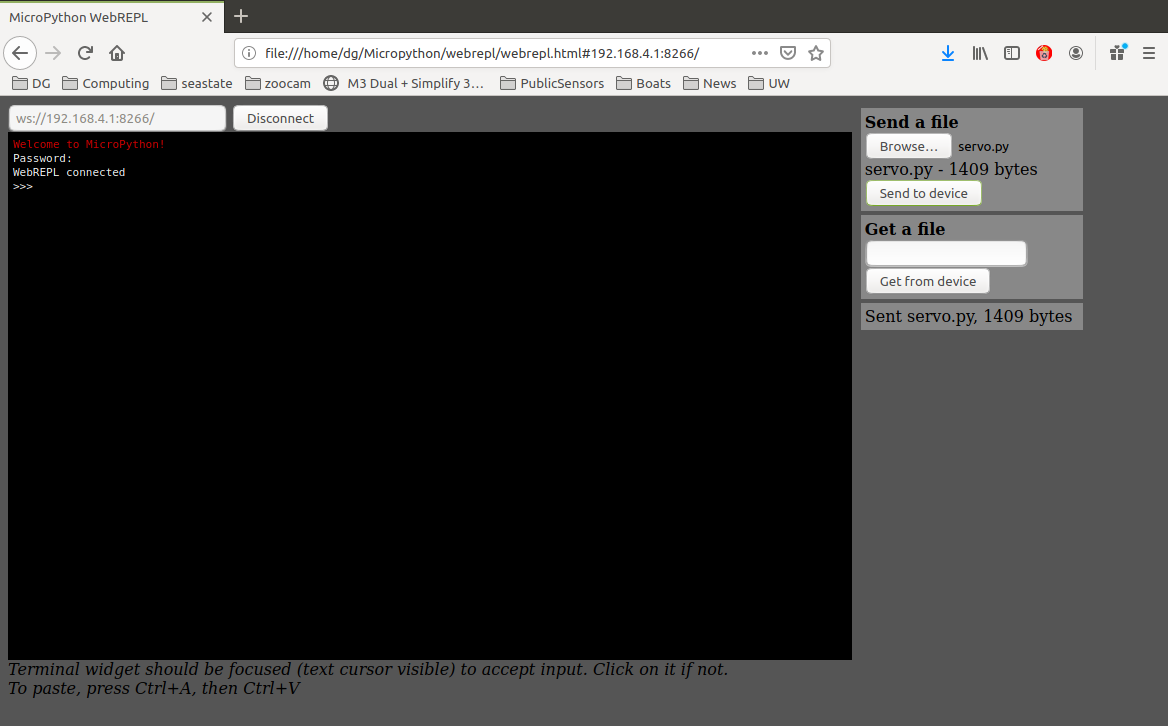
\includegraphics[width=\MFW]{Images/WebREPLupload2.png}}{https://publicsensors.org/IntroSensors/Images/WebREPLupload2.png}
		\caption[A WebREPL session with upload.]{An active WebREPL session, showing the login prompt (main terminal frame) and a file upload (right side panel.}
		\labfig{WebREPL_upload}
	\end{center}
\end{marginfigure}
\texttt{WebREPL} can do both of the essential elements of communicating with microcontrollers, via a wireless connection:
It provides access to REPL, and makes it very easy to upload and download files between your laptop and the ESP8266 (\reffig{WebREPL_upload}).

%Note: Your microcontroller has to be connected via wifi for WebREPL to work, either with your laptop logged onto an Access Point created by the microcontroller, or with both your laptop and microcontroller logged onto another Access Point.

WebREPL is a free download from this	 \htmladdnormallink{link}{https://github.com/micropython/webrepl}. \sidenote[][*6]{\begin{kaobox}[backgroundcolor=\SNcolor,frametitlebackgroundcolor=\SNcolor,frametitle=Locally sourced\dots]\texttt{WebREPL} is available to use online, without installing it.
\emph{However, you will most likely want to have it actually installed directly on your computer.}
That is because, unless you have multiple internet connections available on your computer, you can’t use the online WebREPL when you connect directly to your ESP8266 as an Access Point.
You can, however, use the online \texttt{WebREPL} if your laptop and microcontroller are both logged onto another Access Point.
We recommend installing \texttt{WebREPL} on your computer because in the upcoming activities you will likely have your microcontroller connected as a station and as an access point at various times.\end{kaobox}}

An easy way to install the WebREPL archive on your machine is downloading the \htmladdnormallink{zipped package}{https://github.com/micropython/webrepl/archive/master.zip}.
Some useful introductory information on using WebREPL is provided by Adafruit
\htmladdnormallink{here}{https://learn.adafruit.com/micropython-basics-esp8266-webrepl/access-webrepl},
\htmladdnormallink{here}{https://learn.adafruit.com/micropython-basics-esp8266-webrepl/overview} and
\htmladdnormallink{here}{https://learn.adafruit.com/micropython-basics-esp8266-webrepl/send-and-get-files}.
%\begin{verbatim}
%https://learn.adafruit.com/micropython-basics-esp8266-webrepl/access-webrepl
%https://learn.adafruit.com/micropython-basics-esp8266-webrepl/overview
%https://learn.adafruit.com/micropython-basics-esp8266-webrepl/send-and-get-files
%\end{verbatim}


\subsubsection{\howto Launch WebREPL on your computer}
\begin{enumerate}
	\item  \textbf{Open the file \texttt{webrepl.html} in the \texttt{webrepl} directory}
	This is the directory that you unzipped from the archive you downloaded from \texttt{github}.
	WebREPL should work equally well in Chrome, Firefox, Chromium, Opera and other browsers.
	You should see a window like \reffig{WebREPL_upload} appear in your browser.

	\item \textbf{If necessary, enter your microcontroller's IP number in the text box at the upper left}.

	The text box at the upper left has an address that looks like
\begin{lstlisting}[language=bash]
ws://192.168.4.1:8266
\end{lstlisting}
	This has three parts:
	\begin{itemize}
		\item The first item, \verb|ws|, stands for \texttt{websocket}, the format for connecting.

		DON'T CHANGE THIS!

		\item The last item, \verb|8266|, is the port number over which to connect.

		DON'T CHANGE THIS EITHER!

		\item The middle item, \verb|192.168.4.1|, is the IP number for your microcontroller.

		There are two cases here:
	\begin{itemize}
		\item \textbf{If you are connecting to your microcontroller using its own \texttt{AP} mode, then you don't have to change anything.} The default, \verb|192.168.4.1|, is already correct.

		\item \textbf{If you are connecting to your microcontroller using its \texttt{STA} mode with a router, you will likely need to change the IP number in this box to reflect the IP assigned by the router to your ESP8266.} This is the first entry in the result of the \texttt{wlan.ifconfig()} command above.

		If you need to change the IP number, be careful not to accidentally change either of the other two items.
		If you do happen to change them, you can easily recover the defaults by pressing the reload button on your browser window.
	\end{itemize}
	\end{itemize}


	\item \textbf{Click “Connect” and enter your password after the prompt.}

	You should see the new connection reflected in a \verb|>>>| python prompt.

\end{enumerate}

%Summary: 1) Open webrepl.html in a browser; 2) Enter IP number in text box; 3) Click Connect \& enter password

%\marginnote[0cm]{
\begin{kaobox}[frametitle=Making sure \texttt{webrepl} is active on your microcontroller \dots]
\texttt{WebREPL} has two parts:
One is the web page that you open on your laptop.
The other is a Python script called \texttt{webrepl} (note the lower case!) that runs on your microcontroller.
\texttt{webrepl} must be activated for you to connect through \texttt{WebREPL}.

There are a couple of important details in making sure that \texttt{webrepl} is activated on your microcontroller:
\begin{itemize}
\item \textbf{The first time you want to connect via \texttt{WebREPL}, you need to initialize \texttt{webrepl} (set a password, \etc) by using your USB connection to issue the command}
\begin{lstlisting}[language=Python]
import webrepl_setup
\end{lstlisting}
Three things then happen:
\begin{itemize}
	\item The microcontroller will ask whether you want to ``enable'' \texttt{webrepl} (automatically start it each time the microcontroller reboots). Enter \texttt{E} to enable.
	\item The microcontroller will prompt you for a password, which you need to enter twice.
	\item The microcontroller will ask whether to reboot, which is necessary to implement your new settings (Enter \texttt{y}, for yes).
\end{itemize}
When you have finished these three steps, \texttt{webrepl} is set to start by default with the password you set when you reboot the microcontroller.

\item \textbf{If you are connected to your microcontroller via USB, sometimes \texttt{webrepl} does not run even if you set it to. In that case, you need to use your USB connection to execute the commands}
\begin{lstlisting}[language=Python]
import webrepl
webrepl.start()
\end{lstlisting}
to manually start \texttt{webrepl}. Your microcontroller will then be available to connect via the WebREPL browser window.
\end{itemize}
\end{kaobox}
%}

%\subsubsection{\howto Up- and download files over WiFi with \texttt{WebREPL}}
\texttt{WebREPL} makes it easy to transfer files from your laptop to your microcontroller and \textit{vice versa}:

\subsubsection{\howto Upload a file to your microcontroller using \texttt{WebREPL}}
\begin{enumerate}
	\item \textbf{Click on the \texttt{Browse} button at the upper right of the \texttt{WebREPL} window, under the \texttt{Send a file} prompt} (\reffig{WebREPL_upload}).
	\item \textbf{Navigate to and select the file you want to transfer} (in this example, a file called \texttt{servo.py}).
	\item \textbf{Click the \texttt{Send to device} button.}

	The textbox at the bottom of the right side panel will now report the file sent and the number of bytes uploaded.
\end{enumerate}


\subsubsection{\howto Download a file from your microcontroller using \texttt{WebREPL}}
\begin{enumerate}
	\item \textbf{List the files on the microcontroller with the \Micropython commands:}
\begin{lstlisting}[language=Python]
import os
os.listdir()
\end{lstlisting}

	\item \textbf{\textbf{Enter the name of the file to download in the textbox under the \texttt{Get a file} prompt}} (\reffig{WebREPL_download}).


	\item \textbf{Click the \texttt{Get from device} button.}
	\item \texttt{WebREPL} will download the file, report its name and size in the text box, and prompt you to save or open the file on your laptop.
	\end{enumerate}

\begin{marginfigure}[0cm]
	\begin{center}
		\htmladdnormallink{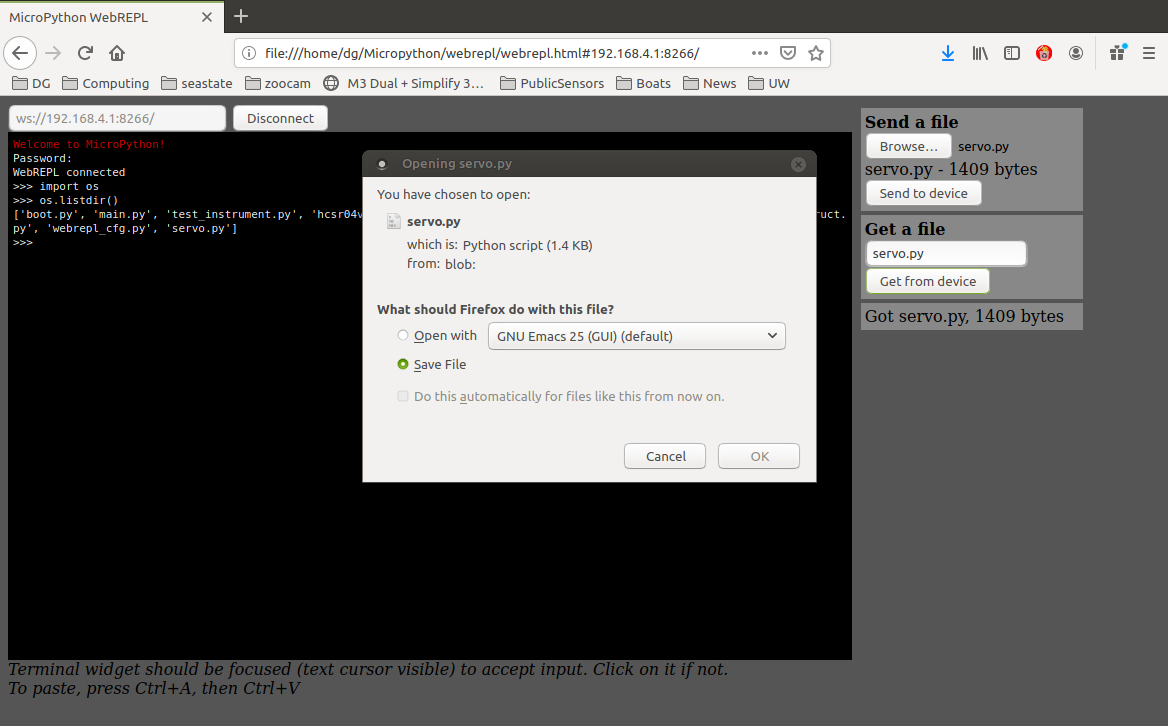
\includegraphics[width=\MFW]{Images/WebREPLdownload.png}}{https://publicsensors.org/IntroSensors/Images/WebREPLdownload.png}
		\caption[A WebREPL session with download.]{An active WebREPL session, showing the commands to list the files on the microcontroller (main terminal frame), a file download (right side panel, and a prompt for how to save or open the file.}
		\labfig{WebREPL_download}
	\end{center}
\end{marginfigure}


%\subsubsection{WiFi connections via \texttt{Secure Shell} in Chrome}
%When your microcontroller is not connected by a USB cable to your laptop, you will connect to it over WiFi.
%If \mpfshell is installed on your  machine, it is likely the best option to connect to your microcontroller over WiFi (see the \htmladdnormallink{mpfshell github site}{https://gist.github.com/hardye/657385210c5d613e69cb5ba95e8c57a7} for instructions on how to connect to a microcontroller via WiFi).
%\texttt{WebREPL} is also a good alternative, but for \texttt{WebREPL} to work it must be enabled on your microcontroller.
%If it is not enabled, and if you prefer a browser-based communication method, you can use an alternative like \htmladdnormallink{Secure Shell}{https://chrome.google.com/webstore/detail/secure-shell/pnhechapfaindjhompbnflcldabbghjo?hl=en} instead.
%
%(including logging onto your microcontroller to enable WebREPL).
%
%in some ways nicer to use than Secure Shell
%
%For this you will need a different app than you used for serial communication – you will need a terminal interface through which you can remotely log onto your microcontroller, to issue commands and obtain sensor readings.
% is an app that provides this capability.
%
%
%
%In many cases you will be able to use WebREPL instead of Secure Shell -- it also enables you to log onto your microcontroller.
%

\subsection{\color{gray}WiFi connections using \thonny\color{black}}

\subsection{WiFi connections using \mpfshell}
\mpfshell is as useful for connecting to your ESP8266 remotely over WiFi as it is for connecting directly via USB.

\subsubsection{\howto Connect with your microcontroller using \mpfshell over WiFi}
\begin{enumerate}
	\item \textbf{Make sure \texttt{webrepl} is enabled (see instructions above for \texttt{WebREPL} if you're not sure).}
	\item \textbf{In a terminal window, launch \mpfshell:}
\begin{lstlisting}[language=Python]
mpfshell
\end{lstlisting}
	\item \textbf{Open the connection over WiFi with}
\begin{lstlisting}[language=Python]
open ws:192.168.4.1
\end{lstlisting}

	In this command, the number \texttt{192.168.4.1} is the microcontroller's IP number.
	If the microcontroller's \texttt{AP} is activated and your laptop is connected to it, this IP number is correct.

	If you are connecting via a router, then you need to replace this number with the IP assigned to your microcontroller (see the \texttt{wlan.ifconfig()} command in the instructions for WebREPL).

	\item \textbf{At the prompt, enter your \texttt{webrepl} password.}

	You should then see the \verb|mpfs [/]>| prompt showing that you have successfully connected through \mpfshell.
\end{enumerate}

All the \mpfshell file transfer and REPL capabilities work the same over WiFi as when connected via USB.

\loadMilestone{mlst:01b} % load milestone with tags id: mlst:01b


\section{Computing on your microcontroller using \Micropython libraries}
\labsec{mp_libs}
The great utility of \Micropython is that it makes programming and interacting with environmental sensors quick and effective.
An additional feature is that \Micropython contains many useful libraries that you can use ``out of the box'', without any external hardware.
A good source for examples and advice on using \Micropython is the \htmladdnormallink{Micropython forum}{https://forum.micropython.org/viewforum.php?f=16&sid=3b047a13be25c6522d788bfb036217a6}.
To conclude this first chapter on communicating with your microcontroller, you will implement two examples from this forum that illustrate how to generate random numbers, and how to encrypt a string of characters.
You will then anticipate later chapters in which you will telemeter environmental data over publicly available websites, by implementing a basic form of data verification.

\subsection{Generating random numbers and strings}
\labsec{rnd}
Random numbers and strings are useful for a variety of purposes in scientific data analysis and modeling.
Later in this section, we will use randomized strings to make environmental data transmissions easier to verify.
Micropython has a built-in utility, \lstinline{getrandbits} in the \lstinline{urandom} library, to generate random bits.
These random bits can then be converted into random numbers and strings. Here's how to do it:

\subsubsection{\howto Generate random numbers and strings}
A post on the \htmladdnormallink{Micropython forum}{https://forum.micropython.org/viewtopic.php?t=6158} provides an easy-to-use function that converts random bits bits into random integers in a user-supplied range.
\begin{enumerate}
	\item \textbf{To generate random integers, download} the \lstinline{random_int.py} \textbf{python script by clicking on the link in the margin. Then, use the \lstinline{<ctrl>-e/<ctrl>-d} technique to paste the following commands into a \texttt{REPL} session:}
	\lstinputlisting[language=Python,label=random_int,caption={\htmladdnormallink{\texttt{random\textunderscore int.py}}{https://github.com/publicsensors/IntroSensors/blob/main/Codes/random_int.py}: A Micropython script demonstrating generation of random integers within a specified range.}]{Codes/random_int.py}

	This code defines a function, \lstinline{randint}, that returns a single random integer between the input parameters \texttt{min} and \texttt{max} (including \texttt{min} and \texttt{max}).

	Try generating a list of random integers with a command like
\begin{lstlisting}[language=Python]
print([randint(0,999) for i in range(45)])
\end{lstlisting}
	Were you successful in generating random integers?

	\item \textbf{Generate random strings by random selections from a list of characters.}

	First, define a string containing the list of characters from which to select.
	As an example, we'll use the 26 lower case letters in the English alphabet:
\begin{lstlisting}[language=Python]
char_list=['a','b','c','d','e','f','g','h','i','j',\
           'k','l','m','n','o','p','q','r','s','t',\
           'u','v','w','x','y','z']
\end{lstlisting}
	Now, use these commands to generate a random sequence of the characters in \lstinline{char_list} that is \lstinline{str_len} letters long:
\begin{lstlisting}[language=Python]
str_len=20
rnd_str=''.join([char_list[randint(0,len(char_list)-1)] for i in range(str_len)])
print(rnd_str)
\end{lstlisting}
	In these commands, \lstinline{randint(0,len(char_list)-1)} randomly chooses the index of a character in \lstinline{char_list}.
	After this is repeated \lstinline{str_len} times to form a list of characters, the list is joined into a single string.

	Repeat these commands several times with different character lists and \lstinline{str_len} values to demonstrate that you are successfully generating random strings.

\end{enumerate}
\loadMilestone{mlst:01c} % load milestone with tags id: mlst:01c


\subsection{Encryption of character strings}
\labsec{encrypt}
\Micropython comes equipped with a basic encryption library called \lstinline{ucryptolib}.
This library is modeled after the larger  Python library \lstinline{cryptolib}, but is more limited so that it can run on microprocessors rather than full sized computers.
The encryption methods used in this library are not safe enough to be used for truly sensitive information -- with effort, they can be decrypted by an expert hacker.
Furthermore, the ``key'' to reading the data is stored on the microcontroller, so someone with physical access to the instrument could easily decrypt messages.
However, in most of our applications it's not worth anyone's trouble to decrypt environmental sensor data -- and in any case, it's not usually a secret.
The more important issue for us is being able to know that a message appearing to contain data from our sensor is genuine.
For this purpose, it's sufficient to include an encrypted password or token that an unauthorized sender is unlikely to know.

\subsubsection{\howto Encrypt and decrypt messages on your microcontroller}
With this relatively low standard of encryption in mind, let's demonstrate a basic use of \lstinline{ucryptolib} posted on the Micropython forum by \htmladdnormallink{@jimmo}{https://forum.micropython.org/viewtopic.php?t=6726}.
\begin{enumerate}
	\item \textbf{To encrypt strings, download} the \lstinline{encrypt_demo.py} \textbf{python script, and use the \lstinline{<ctrl>-e/<ctrl>-d} technique to paste the following commands into a \texttt{REPL} session:}
\lstinputlisting[language=Python,label=encrypt_demo,caption={\htmladdnormallink{\texttt{encrypt\textunderscore demo.py}}{https://github.com/publicsensors/IntroSensors/blob/main/Codes/encrypt_demo.py}: A Micropython script demonstrating simple encryption of short strings.}]{Codes/encrypt_demo.py}

	In this example,the string \texttt{input plaintext} is first placed into the variable \lstinline{data}.
	The string is then converted to bytes, and stored as the variable \lstinline{data_bytes}.

	\smallskip
	For this encryption method, the input string must be packaged in ``blocks'' of 16 bytes.
	This means that long messages must be split into shorter messages of 16 or fewer bytes, and that shorter messages must be ``padded'' by tacking on additional bytes to meet the length requirement.
	This is done in the example above by the modification of \lstinline{data_bytes} into \lstinline{data_bytes16}.
	The modified characters from the original string are then encrypted using the \lstinline{encrypt} function from \lstinline{ucryptolib}.

	\smallskip
	These steps are then repeated for the second string, \texttt{input pl}.

	The output from these commands should be
\begin{lstlisting}[language=Python]
msg1 =  b'\xfe!F\x87?\xdb\x19\x18\xcdM\x83\x9b\xaa\x02\xa9\x04'
msg2 =  b"[\x9df\xa3\xa0\xa5'\xa5v\xc1\xfeNI\xa9\x96\x03"
\end{lstlisting}
	These messages could be conveyed in a public venue, and without knowing or guessing the key (not very hard in this example) it would be difficult --- but not impossible --- for an eavesdropper to extract the original strings.

	\item \textbf{To decrypt strings, download} the \lstinline{decrypt_demo.py} \textbf{python script, and use the \lstinline{<ctrl>-e/<ctrl>-d} technique to paste the following commands into a \texttt{REPL} session:}
\lstinputlisting[language=Python,label=decrypt_demo,caption={\htmladdnormallink{\texttt{decrypt\textunderscore demo.py}}{https://github.com/publicsensors/IntroSensors/blob/main/Codes/decrypt_demo.py}: A Micropython script demonstrating simple decryption of short strings.}]{Codes/decrypt_demo.py}

	In this command sequence, the key is used to decrypt \lstinline{msg1} and  \lstinline{msg1} into the bytes from which they were generated.
	Those bytes are then converted back to strings, and the ``padding'' characters \lstinline{\x00} are removed (``stripped'')).

	The output from the decryption commands should be
\begin{lstlisting}[language=Python]
data1= input plaintext
data2= input pl
\end{lstlisting}
	which successfully recovers the original messages.

	\item \textbf{Try it with your own key and messages, taking care to split messages longer than 16 characters into shorter ones.}

	Assuming that \lstinline{\x00} was not part of the original messages, your own key should enable you to encrypt and decrypt your messages.
	If you want to include \lstinline{\x00} in your messages, you can substitute a different character as padding that does not appear in your messages.
\end{enumerate}


\subsection{Encrypted authentication of data messages}
In most uses of environmental sensors, the acquired data is not a major security concern.
That is, if we post e.g. a temperature reading to a publicly accessible website, there is usually little harm done.
Ideally, the data are relevant and well enough presented that they are helpful to other readers.
However, there is a concern if posting data makes it too easy for a viewer to mimic true data uploads by simply copying and pasting corrupted versions of past posts.
The form of encryption from \refsec{encrypt}, even though it is not unbreakable, is in general sufficient to provide a means of verifying that data uploads are genuine.

Let's consider a data message of the form
\begin{lstlisting}[language=Python]
Instrument1,Sensor3,watertemp,NorthLakeWashingtonWA,3711,2020-3-19 1:20:17,7.6875
\end{lstlisting}
from an environmental sensor similar to one you will build in later chapters of this book.
In this message, \lstinline{Intrument1} is a label for a particular \texttt{instrument}, i.e., a microcontroller that may have attached a variety of sensors.
\lstinline{Sensor3} indicates the particular sensor from which the reported datum was measured.
\lstinline{watertemp} indicates that water temperature is the environmental characteristic being measured.
\lstinline{NorthLakeWashingtonWA} is a geographical reference readable and specific enough to potentially make the data useful to others.

The actual data, in the part of the message that reads \lstinline{3711,2020-3-19 1:20:17,7.6875}, are the sample number (here, the 3711\textit{th} sample), the date/time stamp, and the temperature reading ($7.6875^\circ$).
Local residents, fishermen, limnologists and many others might find real-time reporting of water temperature from North Lake Washington to be of interest.
This is particularly true if the data from this sensor can be easily put in context with other data such as air temperature, insolation, wind speed and direction, data from elsewhere on Lake Washington, \etc

The key issue is to insure that data from another source that accidentally or intentionally look very similar to this line of data do not mistakenly get accepted into the database for this instrument.

Suppose we take a non-repeating part of this message and encrypt it, together with a \htmladdnormallink{``salt''}{https://en.wikipedia.org/wiki/Salt_(cryptography)}.
In cryptography, a salt is a string of random characters that make encrypted information like passwords harder to guess.
In our case, the sample number is always incremented after a sample, so no two samples will have the same number.
This means that even if the salt and environmental data don't change, the encrypted block will be different for every message.

We will include both the encrypted and plaintext versions of the message in the data line.
Then, any reader who can see the message can get access to the data.
However, only those with the encryption key -- us, because we placed the key on the instrument -- can decrypt the encrypted part of the message.

When we receive a message purporting to come from our instrument, we can decrypt the encrypted part of the message.
If the encrypted sample number matches the reported sample number, the message must have come from our instrument.

An eavesdropper could then resend a data message, combining our encrypted block with bogus data.
However, if that message contains a previously used sample number, we know it is bogus because we have already received data for that sample number.
If the message contains a different sample number, the encrypted and plaintext version won't match and we again know it is bogus.


\subsubsection{\howto Verify a data message}
This is a simple implementation of this message verification strategy:
\begin{enumerate}
	\item \textbf{To augment a message using encryption for verification, download} the \lstinline{encrypt_msg.py} \textbf{python script, and use the \lstinline{<ctrl>-e/<ctrl>-d} technique to paste the following commands into a \texttt{REPL} session:}
	\lstinputlisting[language=Python,label=encrypt_msg,caption={\htmladdnormallink{\texttt{encrypt\textunderscore msg.py}}{https://github.com/publicsensors/IntroSensors/blob/main/Codes/encrypt_msg.py}: A Micropython script demonstrating a simple strategy for augmenting a data message using encryption for verification.}]{Codes/encrypt_msg.py}

	In this example, both the key and the salt are strings of random letters, generated as in \refsec{rnd}.
	The key is 16 characters long (as required by the encryption algorithm), and the salt is 10 characters long so that when the sample number is added the total number of characters will not exceed 16 (we do not expect to take more than 999,999 samples!).

	In a real application, this code would be executed by the microcontroller in an instrument in the field.
	The output, in this example, is the augmented data message
\begin{lstlisting}[language=Python]
Instrument1,Sensor3,watertemp,NorthLakeWashingtonWA,3711,2020-3-19 1:20:17,7.6875,b'$\\xd8\\xd8\\xa5\\x93D\\xd1\\xb3\\xd9=\\xa8$x\\xf6n\\xce'
\end{lstlisting}
	where the rightmost entry in quotes is the encrypted block.

	\item \textbf{To verify the message using decryption, download} the \lstinline{decrypt_msg.py} \textbf{python script, and use the \lstinline{<ctrl>-e/<ctrl>-d} technique to paste the following commands into a \texttt{REPL} session:}
\lstinputlisting[language=Python,label=decrypt_msg,caption={\htmladdnormallink{\texttt{decrypt\textunderscore msg.py}}{https://github.com/publicsensors/IntroSensors/blob/main/Codes/decrypt_msg.py}: A Micropython script demonstrating decryption of an augmented data message for verification.}]{Codes/decrypt_msg.py}

	In a real application, this code would be executed on the receiving machine.
	In this demonstration, you can run it from within the \texttt{REPL} session on your microcontroller or in a Python session on your computer.

	\smallskip
	This code begins by finding the rightmost comma, and using it to separate the original message from the encrypted block.
	It then converts that block from a string back to bytes, and uses the key to decrypt it.
	This is the key verification step, because only the sender and receiver know the key.

	\smallskip
	The code then strips away the padding, and removes the salt by extracting only the digits.
	The string of digits is converted back to an integer.
	If that integer agrees with the sample number in the data, the originator of this message must have had the encryption key, and therefore be legitimate.

	\smallskip
	Note that, like most authentication schemes, this assumes that the key has not been shared and is not easy to guess.
	Furthermore, it assumes that the sample numbers are used only once, and that subsequent data lines reusing a sample number are ignored.
	Otherwise, a reader without the key could just copy both the sample number and the encrypted block, to generate a bogus but apparently verifiable data message.

\end{enumerate}
